\documentclass[conference,10pt]{IEEEtran}
\IEEEoverridecommandlockouts
\usepackage{graphicx,booktabs,amsmath,amssymb,multirow,xcolor,url,xspace}
\usepackage[hidelinks]{hyperref}
\hypersetup{pdftitle={로봇 양팔을 위한 에고센트릭 인간 시연, 제1부: 큐브 삼단 쌓기}, pdfauthor={Jeong Hwan Lee}}
\usepackage{tikz}
\usetikzlibrary{positioning,arrows.meta,fit,backgrounds}
\usepackage{fontspec}\setmainfont{Times New Roman}\usepackage{xeCJK}\setCJKmainfont[AutoFakeBold=2.5]{AppleMyungjo}\setCJKsansfont[AutoFakeBold=2.5]{Apple SD Gothic Neo}\setCJKmonofont{Apple SD Gothic Neo}\xeCJKsetup{CJKecglue={},CJKspace=true}
\newcommand{\mm}{\,mm\xspace}
\newcommand{\cmt}[1]{}

\begin{document}
\title{로봇 양팔을 위한 에고센트릭 인간 시연\\제1부: 큐브 삼단 쌓기}
\author{\IEEEauthorblockN{Jeong Hwan Lee}
\IEEEauthorblockA{기술 보고서, 버전 4, 2026년 10월 7일 \quad alnrg2arg@gmail.com\\
제2부는 단일 팔 접근(approach) 데이터를 다룹니다. 코드, 결과, 샘플 데이터는 요청 시 제공합니다.}}
\maketitle

\begin{abstract}
본 연구는 손에 착용하는 UMI 방식 그리퍼로 기록한 자연스러운 에고센트릭(egocentric) 인간 시연을 양팔 로봇 정책의 학습
데이터로 어디까지 바꿀 수 있는지 살펴본다. 양손 손목 어안(fisheye) 카메라, IMU, 조(jaw) 인코더와 고정 헤드 카메라를 사용하여,
수집 시점에 균형을 맞춘 여섯 가지 쌓기 순서(순서당 51--64 에피소드)로 큐브 세 개를 쌓는 과제의 양팔 시연 349개를 수집하였다.
다단계 파이프라인(에피소드별 시각--관성 스케일을 적용한 MASt3R-SLAM 손목 자세, 6-DoF 로봇 팔로의 리타게팅, 그리고 동기화·작업공간·
메트릭·역기구학 게이트)을 거쳐 259개 에피소드, 즉 65프레임 양팔 세그먼트 561개가 남는다. 이 데이터로 0.9B 파라미터
vision-language-action 모델(X-VLA)을 파인튜닝하여 30스텝 관절 공간 액션 청크를 예측하게 하고, held-out 에피소드 26개에서
오프라인으로 평가하였다. held-out TCP 오차의 중앙값은 0.2--1.2\,s 구간에서 1.5--5.7\mm{}이다. 이 수치는 정지 구간이 지배한다.
목표가 20\mm 이상 움직이는 23\%의 샘플에서는 1.2\,s 시점 오차가 39.9\mm, 방향 코사인이 0.90이며, 정책은 무동작 예측기 대비 관절
오차를 24\% 줄인다. 순서 지시문을 바꾸면 예측 동작이 측정 가능한 수준으로 변하지만 그 크기의 ${\sim}8\%$에 불과하며, 올바른
지시문이 틀린 다섯 개 지시문보다 인간 동작을 더 잘 예측하지 못한다. 따라서 이 평가에서 모델은 순서 지시문을 과제에 유용한
방식으로 사용하지 않는다.
두 후속 실험은 주요 병목을 다룬다. 단일 앵커 리타게팅을 다중 시드 궤적 윈도 검색(retrieval)으로 바꾸면 사용 가능한 후보 세그먼트
비율이 36.5\%에서 56.1\%로 오르고, 리타게팅된 자세가 실제 로봇 자세에 훨씬 가까워진다. 수집 방식이 리타게팅 가능성을 바꾸는지
검증하기 위해 60개 에피소드를 로봇 유사 방식으로 재수집하였으나, 눈에 띄는 변화는 없었다(부정적·진단적 결과). 로봇 시연 150개로
파인튜닝했을 때, 에고 사전학습 모델의 geo score는 다른 조건이 동일한 처음부터 학습한(scratch) 모델보다 10\% 낮다(95\% CI 5.6--14.7\%).
단, 이는 두 학습 세트 모두에 포함된 에피소드에서만 측정한 것이다.
이번 버전은 관절 공간 리타게팅을 아예 없앤 세 번째 단계를 추가한다. 인간 에피소드 전체를 로봇 데이터와 같은 20차원 배치의
상대 데카르트(Cartesian) 엔드이펙터 액션으로 변환하며, 작업공간이나 IK 필터링은 하지 않는다(330 에피소드, 자세 점프 필터 후
학습 행 48{,}411개). 공개 X-VLA base를 점검한 결과 도메인 soft prompt 슬롯 30개 중 8개만 학습된 적이 있었으며, 이는 이전 실행
결과의 해석을 바꾼다. 로봇 카메라 프레임에서 에고 전용 모델은 유용한 동작 방향을 예측하지 못한다(코사인 중앙값 $-0.05$/$-0.03$,
로봇으로 학습한 모델은 $+0.81$/$+0.77$). 도메인 간에 이미지와 상태를 맞바꾸어 보면 격차는 손목 이미지에 있으며, 두 도메인의 손목
이미지 선명도는 약 30$\times$ 차이 난다. 로봇 파인튜닝의 초기값으로 쓰면 에고 모델은 3.9$\times$ 낮은 학습 손실에서 출발하지만,
다른 조건이 동일한 실행에서 60k 스텝 무렵 그 이점은 동률로 줄어든다. 버전 4는 저데이터 ablation을 추가한다. 로봇 에피소드 30개만으로,
base 모델과 100k·300k 스텝 에고 사전학습 체크포인트에서 시작하는, 다른 조건이 동일한 세 파인튜닝 실행이다. 두 에고 초기화 모두
scratch 학습 손실의 절반 미만에서 출발하며, 그 이점은 약 100k 스텝(100k 스텝 사전학습)과 약 200k 스텝(300k 스텝 사전학습)에서
사라지고, 세 실행 모두 30개 에피소드에 심하게 과적합한다. 이들 중 아직 로봇에서 실행된 것은 없다. 로봇 에피소드 312개로 파인튜닝한
에고 초기화 모델은 폐루프에서 큐브 세 개를 끝까지 쌓았으나, 시도 횟수를 세지 않았으므로 성공률이 아닌 시연으로만 보고한다. 새로운
공간 배치나 보지 못한 쌓기 순서를 검증하는 실험은 없으며, 이 데이터가 뒷받침할 수 있는 주장과 없는 주장을 명시한다. 버전 3의
제XII절이었던 단일 팔 접근 연구는 이제 제2부가 되었다.
\end{abstract}

\section{서론}\label{sec:intro}
로봇 시연 수집은 실제 로봇, 조작자, 과제별 원격조작 인프라가 필요하여 대개 비용이 크다. 에고센트릭 인간 시연은 더 적은 하드웨어로,
자연스러운 환경에서, 더 빠르게 수집할 수 있으며, UMI~\cite{chi2024umi}와 같은 손 착용 그리퍼는 인간의 엔드이펙터를 로봇과 비슷하게
만들어 그리퍼 수준의 embodiment 격차를 줄인다. 이러한 데이터가 특정 로봇으로 전이되는지는 처음부터 끝까지 점검되는 일이 드문
일련의 단계에 달려 있다. 센서 캘리브레이션, 움직이는 손목 카메라로부터의 메트릭 자세 복원, 로봇 기구학으로의 리타게팅, 그리고
어떤 인간 동작을 남길지 결정하는 필터링이다. 각 단계는 정책이 결국 무엇을 학습하는지를 드러나지 않게 바꿀 수 있다.

본 보고서는 실제 데이터로 이 사슬을 한 번 완주한 과정을 기록하고, 의도적으로 좁은 질문을 던진다.
\emph{모든 처리를 거친 뒤, 사전학습된 vision-language-action(VLA) 모델은 리타게팅된 에고센트릭 인간 시연으로부터 로봇이 실행 가능한
액션 구조를 얼마나 학습하며, 과제 순서 지시문을 사용하는가?} 기여는 다음과 같다.
\begin{itemize}
\item 여섯 가지 균형 잡힌 쌓기 순서로 구성된 큐브 삼단 쌓기 양팔 에고센트릭 데이터셋 349 에피소드와 전체 센서 캘리브레이션 및
에피소드별 메타데이터(\ref{sec:data}절)
\item 원시 인간 영상에서 로봇 관절 공간 세그먼트에 이르는 처리 퍼널(funnel)을 문서화하고 각 게이트가 무엇을 제거하는지 보고
(\ref{sec:proc}절)
\item 그 결과로 파인튜닝한 0.9B 파라미터 VLA의 오프라인 평가. 집계 오차가 정지 구간에 지배됨을 보이는 동작 게이트 분석과
지시문 사용 여부를 검증하는 prompt swap 실험을 포함(\ref{sec:eval}--\ref{sec:fail}절)
\item 리타게팅 병목, 로봇 유사 재수집, 에고→로봇 파인튜닝에 관한 후속 실험(\ref{sec:follow}절)
\item 로봇의 액션 계약(contract)에 맞춘 에피소드 전체의 데카르트 변환과 그로써 드러난 자세 점프 실패(\ref{sec:v3}절), 그리고
시각·상태·초기화 효과를 분리하는 전이 진단(\ref{sec:transfer}절)
\item 로봇 에피소드 30개에서의 에고 사전학습 길이에 대한 저데이터 ablation(\ref{sec:r30}절)
\end{itemize}
범위를 분명히 해 둔다. 평가는 held-out \emph{에피소드}에 대한 개루프 평가이며 폐루프 로봇 시험이 아니다. 또한 배치가 기록되지
않았고 여섯 순서 모두 학습에 등장하므로 공간 일반화도 과제 순서 일반화도 측정하지 않는다. \ref{sec:intro}--\ref{sec:follow}절은
실행 상태를 제외하면 버전 2(2026년 9월 30일)와 내용상 같고, \ref{sec:v3}--\ref{sec:transfer}절은 버전 3(2026년 10월 4일)과 같으며,
\ref{sec:r30}절은 새로 추가되었다. 버전 3에는 단일 팔 접근 연구도 있었으나 별도 보고서(제2부)로 확장되었으며, 제2부는 여기서 설명하는
장치, 자세 파이프라인, 액션 계약을 재사용한다. \ref{sec:lim}절에는 본 보고서가 하지 않는 주장에 필요한 실험을 정리한다.

\section{관련 연구 및 동기}
\textbf{휴대형 시연 인터페이스.} UMI~\cite{chi2024umi}는 손목 어안 카메라로 손에 든 그리퍼 시연을 기록하고, 장면별 지도에 대해
ORB-SLAM3로 자세를 복원한다. DexCap~\cite{wang2024dexcap} 등 관련 시스템은 다지 손을 대상으로 한다. 본 장치는 UMI의 손목 카메라
설계를 따르되 손마다 IMU와 조 인코더를, 그리고 고정 헤드 카메라를 추가하였다.
\textbf{에고센트릭 인간으로부터의 학습.} EgoMimic~\cite{kareer2024egomimic}과 MimicPlay~\cite{wang2023mimicplay}는 인간 에고센트릭
영상과 로봇 데이터로 로봇 정책을 공동 학습하며, Ego4D~\cite{grauman2022ego4d}와 같은 대규모 에고센트릭 코퍼스는 스케일링 논거의
동기가 된다. 이들 연구는 폐루프 성능 향상을 보고하는 반면, 본 연구는 처리 후 무엇이 남고 모델이 오프라인에서 무엇을 학습하는지를
점검하며, 이는 그러한 향상을 해석하기 위한 전제 조건이다.
\textbf{정책.} 액션 청킹 모방 학습(ACT~\cite{zhao2023act}, Diffusion Policy~\cite{chi2023diffusion})과 VLA 모델
(OpenVLA~\cite{kim2024openvla}, $\pi_0$~\cite{black2024pi0}, X-VLA~\cite{zheng2025xvla})은 이미지와 언어로부터 다단계 액션 청크를
예측한다. 본 연구는 LeRobot~\cite{cadene2024lerobot}을 통해 X-VLA를 사용하는데, flow matching~\cite{lipman2023flow} 헤드와
soft prompt가 작은 데이터셋으로도 새 embodiment를 수용하기 때문이다.
\textbf{자세 복원.} MASt3R-SLAM~\cite{murai2025mast3rslam}은 3D 복원 사전지식으로 조밀한 단안 SLAM을 제공한다. 본 연구는 이를
Kalibr~\cite{furgale2013kalibr}로 캘리브레이션한 IMU 기반 스케일 추정과 결합한다.

\begin{figure*}[t]
\centering
\begin{tikzpicture}[font=\scriptsize, node distance=3.5mm and 3.5mm,
  box/.style={draw=black!55, rounded corners=1.5pt, align=center, inner sep=2.5pt, minimum height=9.5mm, text width=23mm, fill=white},
  gate/.style={box, fill=orange!8, draw=orange!60!black},
  learn/.style={box, fill=blue!7, draw=blue!55!black},
  arr/.style={-{Stealth[length=1.6mm]}, draw=black!60}]
\node[box] (dev) {\textbf{HandUMI 장치} (양손)\\손목 어안 1080p30, IMU 200\,Hz, 조 인코더; 헤드 카메라 640$\times$480};
\node[box, right=of dev] (cal) {\textbf{캘리브레이션}\\KB 어안, Kalibr 카메라--IMU, 캘리퍼 카메라$\to$TCP, 조 폭};
\node[box, right=of cal] (pose) {\textbf{손목 자세}\\MASt3R-SLAM (RGB) + 에피소드별 IMU--VI 스케일};
\node[box, right=of pose] (ret) {\textbf{리타게팅}\\TCP $\to$ reBot 6-DoF IK 의사 관절, 로봇 시작 앵커};
\node[gate, right=of ret] (qa) {\textbf{QA 게이트}\\동기화 $\le$20\,ms, 작업공간, 메트릭, IK, 세션 격리};
\node[box, below=5mm of dev] (col) {\textbf{수집}\\349 에피소드, 15 세션, 균형 6순서, 20\,s 자동 루프};
\node[box, right=of col] (seg) {\textbf{세그먼트}\\259 에피소드에서 65프레임(2.17\,s) 양팔 561개};
\node[box, right=of seg] (split) {\textbf{분할} (에피소드 단위)\\학습 233 / 검증 26 (504 / 57 세그먼트)};
\node[learn, right=of split] (vla) {\textbf{X-VLA 0.9B} 파인튜닝\\3시점 + 프롬프트 + 14-D 상태 $\to$ 30$\times$$\Delta q$ 청크};
\node[learn, right=of vla] (ev) {\textbf{오프라인 평가}\\FK TCP 오차, 동작 게이트, prompt swap};
\draw[arr] (dev)--(cal); \draw[arr] (cal)--(pose); \draw[arr] (pose)--(ret); \draw[arr] (ret)--(qa);
\draw[arr] (dev)--(col); \draw[arr] (qa.south) |- ++(0,-2.2mm) -| (seg.north);
\draw[arr] (col)--(seg); \draw[arr] (seg)--(split); \draw[arr] (split)--(vla); \draw[arr] (vla)--(ev);
\end{tikzpicture}
\caption{시스템 및 데이터 파이프라인. 주황색: 손실량을 표~\ref{tab:funnel}에 보고한 필터링 단계, 파란색: 학습 및 평가.
어떤 단계도 로봇 롤아웃을 사용하지 않는다.}
\label{fig:pipeline}
\end{figure*}

\section{데이터셋 및 과제 설계}\label{sec:data}
\textbf{하드웨어.} 양손에 각각 HandUMI 장치를 착용한다. 1920$\times$1080, 30\,fps 어안 카메라, 200\,Hz IMU, 100\,Hz로 샘플링하는
조 인코더로 구성된다. 머리에 고정한 Logitech C922가 탁자를 640$\times$480, 30\,fps로 기록하며, 이것이 정책에 주어지는 전역
시점이다(그림~\ref{fig:dataset}a). 모든 스트림은 에피소드마다 MCAP 파일 하나와 영상 세 개로 저장된다.

\textbf{과제.} 50\mm 큐브 세 개(빨강, 파랑, 보라)를 고정된 접시 위에 여섯 순서 중 하나로 쌓는다. 지시문은 순서를 명시하며, 예를 들어
``Stack the blue cube on the bottom, purple cube in the middle, and red cube on the top, on the plate.''이다. 자동 루프가 음성
신호 후 20\,s 테이크를 기록하고, 조작자가 손으로 큐브를 다시 놓는 10\,s의 리셋 시간을 준다. 다음 순서는 가장 적게 수집된 순서(순서당
목표 50개)로 정해지므로, 순서는 무작위가 아니라 \emph{균형}을 맞춘 것이다. 큐브 배치는 수동 리셋을 통해 로봇 작업공간에 맞춘 기준
배치 주변에서 에피소드마다 달라지지만 기록되지 않았으며, 에피소드별 배치 레이블은 없다.

\textbf{수집.} 조작자 한 명이 사흘(2026년 9월 15--17일)에 걸쳐 15개 세션에서 에피소드 349개, 총 2.20\,h(에피소드 중앙값 23.05\,s)를
기록하였다. 순서별로 RBP 64, RPB 62, BRP 61, BPR 56, PRB 55, PBR 51이다(그림~\ref{fig:dataset}b). 초기 10개 세션의 에피소드(55개)는
그리퍼 앵커를 사후에 도출했기 때문에 주 데이터 294개와 별도의 출처 도메인(``early'')으로 관리한다. 필터링 후 두 도메인은 비슷하게
동작한다.

\textbf{캘리브레이션.} 손목 카메라는 Kannala--Brandt 어안 모델을 사용한다(왼쪽 $f_x{=}789$, 오른쪽 $f_x{=}791$\,px). Kalibr 카메라--IMU
캘리브레이션 결과 시간 오프셋은 30.2, 32.8\,ms, 평균 재투영 오차는 6.0, 5.6\,px로 높은 편이며, 이것이 자세 정확도를 별도로 검증하는
이유 중 하나다(\ref{sec:proc}절). 카메라--TCP 변환은 UMI가 CAD 상수를 쓰는 방식을 따라 캘리퍼로 측정한 값 $t=[0, 55.3, 122.5]$\mm{}와
고정된 축 치환을 사용한다. 이 값은 장치 하나에서 측정하여 양쪽에 적용하였다. 조 폭 스케일(개구 $67.5\pm5$\mm)은 50\mm 큐브 파지 영상으로
추정하였으며, 캘리퍼 확인은 아직 남아 있다.

\begin{figure*}[t]
\centering
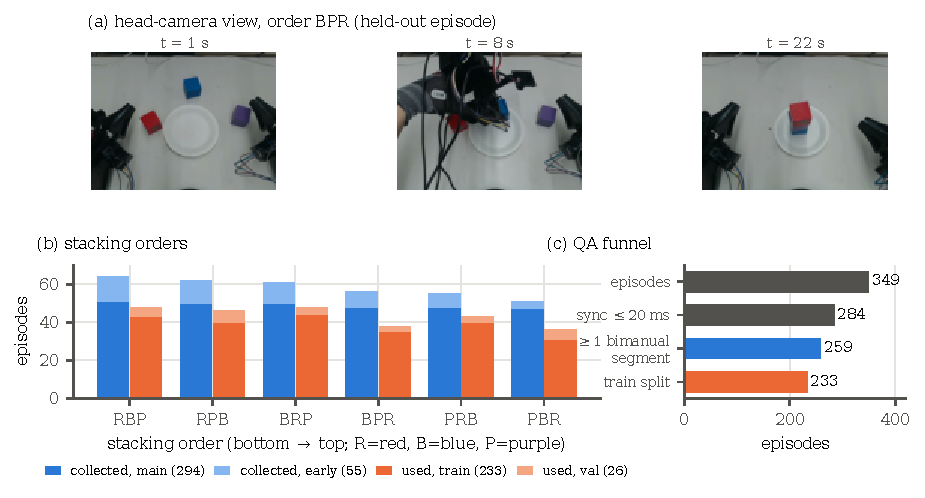
\includegraphics[width=\textwidth]{../figures/fig2_dataset.pdf}
\caption{데이터셋 설계. (a) held-out 에피소드(순서 BPR)의 1, 8, 22\,s 시점 헤드 카메라 프레임. (b) 쌓기 순서별 에피소드 수:
수집 시(main/early 도메인)와 처리 후(학습/검증). (c) 에피소드 수준 QA 퍼널.}
\label{fig:dataset}
\end{figure*}

\section{처리 및 데이터 분할}\label{sec:proc}
\textbf{손목 자세.} UMI는 모든 시연을 장면당 하나의 ORB-SLAM3 지도에서 위치 추정한다. 본 데이터에서는 이 방법이 실패하였다. 장면 변경
전에 만든 지도는 재위치 추정(relocalization)에 실패했고, 마커 벤치마크(아래)에서 그 궤적은 시연당 중앙값 3\%만을 덮었으며 위치 역전이
잦았다(역전율 중앙값 0.24, 채택한 방법은 0.07). 따라서 RGB 손목 영상만으로 MASt3R-SLAM을 실행하고, 에피소드마다 IMU로부터 메트릭
스케일을 복원한다(15프레임 윈도에 대한 시각--관성 피팅). ArUco 마커 에피소드 14개(손 궤적 28개, 그중 10개 held-out)로 이루어진 별도
벤치마크를 데이터셋과 같은 GPU에서 실행한 결과, 추적 커버리지 중앙값은 1.00(저장된 지도를 쓴 ORB-SLAM3는 0.03), 스케일 오차 p50/p90은
4.6/17.0\%(단일 전역 상수는 18.5/23.8\%), 회전 오차 p50/p90은 0.84/2.13\textdegree{}, UMI 방식 16스텝 상대 위치 오차 p90은 11.3\mm{}이다.
349개 에피소드 자체에는 정답(ground truth)이 없다.

\textbf{리타게팅.} 각 TCP 궤적은 URDF 기반 역기구학으로 reBot B601 6-DoF 팔에 매핑된다. 절대적인 작업공간 기하는 에피소드 간에 복원할
수 없으므로, 각 세그먼트를 고정된 로봇 시작 자세(로봇 원격조작 데이터의 활동 자세 중앙값)에 다시 앵커링한다. 즉 동작은 전이되지만 큐브의
절대 위치는 전이되지 않는다. 조 인코더 값은 이진 그리퍼 명령이 된다.

\textbf{게이트.} 표~\ref{tab:funnel}에 퍼널을 정리하였다. 65개 에피소드가 65프레임 전체 윈도에 대한 $\le$20\,ms 동기화 요건을 통과하지
못한다. 나머지 284개에서 양팔 후보 세그먼트 1{,}306개가 나오며, 그중 677개는 로봇 작업공간을 벗어나고, 50개는 메트릭 스케일 검사에, 18개는
IK에 실패하여 561개(43.0\%)가 남는다. 두 세션(에피소드 6개)은 IMU--카메라 회전 불일치로 격리되었으며 세그먼트를 하나도 기여하지 않았다.
학습 단위는 65프레임(2.17\,s) 세그먼트이며, 세그먼트의 47\%가 에피소드 첫 5\,s 안에서 시작한다.

\textbf{분할.} 양팔 세그먼트가 하나 이상인 259개 에피소드를 에피소드 단위로 무작위 분할(seed 0, 10\%)하여 학습 233 / 검증 26, 즉
세그먼트 504/57개, 프레임 32{,}760/3{,}705개로 나눈다. 양쪽에 걸친 에피소드는 없다. 분할은 층화되지 않았으며, 검증 세트는 순서당 3--6
에피소드, main 22 / early 4개이고, 격리되지 않은 13개 세션 중 9개에서 왔다.

\begin{table}[t]
\centering\footnotesize
\caption{처리 퍼널(저장소의 집계 파일로부터 재계산한 수치).}
\label{tab:funnel}
\setlength{\tabcolsep}{4pt}\begin{tabular}{@{}lrr@{}}
\toprule
단계 & 에피소드 & 세그먼트 \\
\midrule
기록됨(KEEP) & 349 & -- \\
자세 + 그리퍼 내보내기(궤적 698개) & 349 & -- \\
동기화 $\le$20\,ms, $\ge$65프레임 윈도 & 284 & 1{,}306 \\
\quad $-$ 작업공간 / 메트릭 스케일 / IK & & $-$677 / $-$50 / $-$18 \\
양팔 세그먼트 $\ge$1개(학습 풀) & 259 & 561 \\
\quad 학습 / 검증(에피소드 단위, seed 0) & 233 / 26 & 504 / 57 \\
\bottomrule
\end{tabular}
\end{table}

\section{모델 및 학습}\label{sec:model}
공개 \texttt{xvla-base} 체크포인트에서 X-VLA~\cite{zheng2025xvla}(LeRobot 구현)를 파인튜닝한다. Florence-2 vision-language
인코더~\cite{xiao2024florence2}와 24층 트랜스포머 정책(hidden 1024, 헤드 16개, soft prompt 32개), flow matching 액션 헤드(디노이징
10스텝)로 구성되며, 파라미터 879M개가 모두 학습 대상이다. 입력은 세 시점(헤드, 왼손목, 오른손목; 224\,px로 리사이즈), 순서 지시문,
14-D 상태(팔마다 관절각 6개와 이진 그리퍼)이다.

\textbf{액션 목표.} 상태 시각 $t$에 대해 모델은 리타게팅된 의사 관절의 누적 관절 변위로 이루어진 30스텝 청크
$a_i = q_{t+5+i}-q_t$, $i=0,\dots,29$를 예측하며(5프레임 선행, 따라서 청크는 0.2--1.17\,s 앞을 덮는다), 여기에 절대 그리퍼 명령을
더한다. 두 보조 항이 관절 공간을 측정된 인간 동작에 묶는다. (C) 측정 궤적의 상대 TCP 위치를 남는 액션 차원에서 예측하는 항(가중치
2.0)과, (D) $\mathrm{FK}(q_t+\hat a_i)$와 측정 TCP 위치 사이의 순기구학 손실(가중치 20)이다. 목표는 측정된 인간 전이이며, 로봇
명령으로 다시 레이블링한 값은 절대 쓰지 않는다.

\textbf{최적화.} 300k 스텝, 배치 4, AdamW(lr $10^{-4}$, weight decay $10^{-4}$, warm-up 1k, $2.5\times10^{-6}$까지 cosine decay),
gradient clipping 10, fp32, RTX~4090 1대. 체크포인트는 10k 스텝마다 저장한다. 체크포인트 선택 규칙, 즉 전체 검증 샘플에 대한
최소 geo score(아래 참조)는 학습 전에 고정하였다.

\section{평가 프로토콜}\label{sec:eval}
평가는 held-out 에피소드 26개에 대한 개루프 평가이다. 검증 세그먼트 57개 각각에서 시작 프레임 7개(0--30 구간에서 5프레임 간격)를
취해 샘플 399개, 팔-샘플 798개를 만들고, 예측 청크를 기록된 미래와 비교한다. 예측 구간 $k\in\{1,4,8,16,30\}$에 대해
$\mathrm{FK}(q_t+\hat a_k)$와 측정 TCP 사이의 TCP 위치 오차(중앙값, mm), 관절 MAE와 \emph{무동작} 예측기($\hat a\equiv0$)의 관절
MAE, 예측·측정 TCP 변위 사이의 코사인을 보고한다. \emph{geo score}는 다섯 예측 구간에 대한 TCP 오차 중앙값의 평균이다. 대부분의
샘플이 거의 정지 상태이므로, 모든 지표를 \emph{동작} 부분집합, 즉 $k{=}30$까지 측정 TCP가 $\ge$20\mm 움직이는 팔-샘플(798개 중
187개, 23.4\%)에 대해서도 보고한다. 이 게이트는 60k 체크포인트를 평가한 뒤에 추가되었으며 보고용으로만 쓴다.

\textbf{Prompt swap.} 지시문 사용 여부를 검증하기 위해 최종 체크포인트에 모든 샘플을 여섯 순서 지시문 각각으로 같은 노이즈 시드를
써서 질의하고, 올바른 지시문으로는 두 개의 추가 시드에서도 질의한다. 여섯 예측의 퍼짐은 지시문의 효과를, 시드 간 퍼짐은 샘플링
노이즈 하한을 나타낸다.

\textbf{분할이 검증하지 않는 것.} 검증 에피소드는 조작자, 장면, 세션, 여섯 순서 전부를 학습과 공유하며, 배치에는 레이블이 없다.
따라서 결과는 새 \emph{에피소드}에 대한 분포 내 일반화를 측정할 뿐, 새로운 배치·순서·장면에 대한 일반화를 측정하지 않는다.

\section{결과}\label{sec:results}
\begin{table*}[t]
\centering\footnotesize
\setlength{\tabcolsep}{7pt}
\caption{오프라인 held-out 결과(에피소드 26개). TCP 오차: FK 위치 오차 중앙값(mm). MAE: 관절 MAE(deg), 괄호 안은 무동작 예측기.
cos: TCP 방향 코사인. 160k는 사전 등록된 선택, 300k는 최종 스텝이다.}
\label{tab:results}
\begin{tabular}{@{}llccccc@{}}
\toprule
 & & \multicolumn{5}{c}{예측 구간 $k$ (5프레임 선행 후 1/30\,s 단위 스텝)} \\
\cmidrule(l){3-7}
부분집합 & 지표 & 1 & 4 & 8 & 16 & 30 \\
\midrule
\multirow{3}{*}{전체 (798)} & TCP 오차, 160k & 1.3 & 1.7 & 2.2 & 3.1 & 5.7 \\
 & TCP 오차, 300k & 1.5 & 1.8 & 2.2 & 3.2 & 5.7 \\
 & MAE, 300k & 0.30 (0.15) & 0.34 (0.19) & 0.42 (0.25) & 0.57 (0.36) & 0.97 (0.51) \\
\midrule
\multirow{4}{*}{동작 (187)} & TCP 오차, 160k & 11.2 & 15.0 & 19.9 & 29.2 & 39.1 \\
 & TCP 오차, 300k & 11.2 & 15.0 & 19.4 & 29.3 & 39.9 \\
 & MAE, 300k & 2.02 (2.32) & 2.68 (3.36) & 3.29 (4.38) & 4.30 (6.34) & 6.59 (8.68) \\
 & cos, 300k & 0.72 & 0.80 & 0.84 & 0.86 & 0.90 \\
\bottomrule
\end{tabular}
\end{table*}

표~\ref{tab:results}와 그림~\ref{fig:eval}에 평가 결과를 요약하였다. 네 가지 결과가 두드러진다.

\textbf{(1) 집계 오차는 주로 정지 구간을 반영한다.} geo score는 160k에서 2.78\mm, 300k에서 2.88\mm{}에 이르며 약 120k 이후로
평탄하다(그림~\ref{fig:eval}a). 그러나 동작 샘플에서는 오차가 한 자릿수 더 크다. 가장 짧은 구간에서 11\mm, $k{=}30$에서 40\mm{}이며
p90은 90\mm{}이다. 동작 부분집합의 geo score는 23.0\mm{}로, 전체 샘플의 2.9\mm{}와 대비된다.

\textbf{(2) 동작 샘플에서 정책은 동작 방향을 예측하며 무동작 기준선을 앞선다.} 방향 코사인은 $k{=}1$의 0.72에서 $k{=}30$의 0.90으로
오르며, 관절 MAE는 모든 구간에서 무동작 예측기보다 13--32\% 낮다($k{=}30$에서 6.59 대 8.68\textdegree{}; 그림~\ref{fig:eval}b).
모델은 다가올 동작의 존재뿐 아니라 그 방향도 포착한다.

\textbf{(3) 전체 샘플에서는 정책이 무동작 예측보다 나쁘다.} 관절 MAE는 모든 구간에서 무동작 MAE의 약 두 배이다($k{=}1$에서 0.30 대
0.15\textdegree{}). 정지 구간에서 정책은 작은 허위 동작을 예측하며, 예측 변위 대 측정 변위 비의 중앙값은 $k{=}1$에서 1.41이다.
$k{=}30$에서 예측의 퍼짐은 목표 퍼짐의 0.77배로, 긴 구간은 붕괴(collapse)되었다기보다 다소 과소 분산(under-dispersed)되어 있다.

\textbf{(4) 순서 지시문은 예측을 바꾸지만 개선하지는 않는다.} Prompt swap(그림~\ref{fig:eval}c)에서 여섯 지시문은 동작 샘플의
$k{=}30$ 예측 TCP를 중앙값 4.8\mm{}만큼 움직이는데, 이는 샘플링 노이즈 퍼짐(0.09\mm)의 약 50$\times$이지만 예측 변위(62\mm)의 8\%에
불과하다. 올바른 지시문이 틀린 지시문보다 기록된 동작에 더 가깝지 않다. 올바른 지시문의 오차는 39.9\mm, 틀린 지시문 평균은 39.5\mm{}이고, 여섯 개
중 평균 순위는 3.55(우연 수준 3.5; 1위 비율 16\%, 우연 수준 17\%)이며, 모든 구간과 전체 샘플에서도 같은 양상이다. 올바른 지시문과 원래
시드로 얻은 예측은 기준 평가를 $10^{-5}$\mm 이내로 재현한다. 한 가지 단서는 2.2\,s 세그먼트의 상당 부분(뻗기, 들어 올리기)이 순서와
무관하다는 점이다. 선택 지점(에피소드의 첫 뻗기)으로 한정한 검증에는 검증 에피소드 26개가 제공하는 것보다 많은 샘플이 필요하다.

순서별 세부 결과는 저장소에 있다. 순서당 검증 에피소드가 3--6개뿐이어서 순서 간 순위를 매기기에는 너무 적으므로, 그 차이는 해석하지
않는다.

\begin{figure*}[t]
\centering
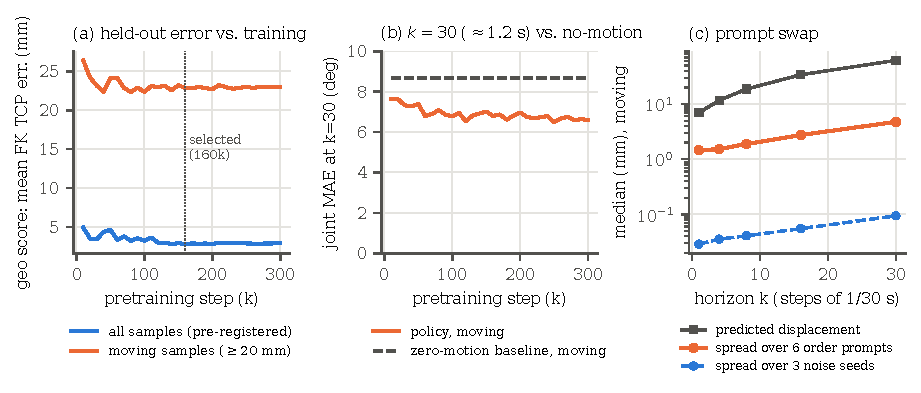
\includegraphics[width=\textwidth]{../figures/fig4_eval.pdf}
\caption{오프라인 평가. (a) 학습 과정에 따른 전체 대 동작 held-out 샘플의 geo score. 사전 등록 규칙은 160k를 선택한다.
(b) 동작 샘플의 $k{=}30$ 관절 MAE, 정책 대 무동작 예측기. (c) 최종 체크포인트에 대한 prompt swap: 여섯 순서 지시문(같은 시드)
간 예측 퍼짐 대 세 노이즈 시드(올바른 지시문) 간 퍼짐.}
\label{fig:eval}
\end{figure*}

\section{실패 분석}\label{sec:fail}
\textbf{과제 순서 지시문의 약한 사용.} 순서 프롬프트는 예측을 측정 가능한 수준으로 바꾸지만, 이 변화가 기록된 동작과의 일치도를
높이지는 않는다(결과 4). 이 데이터셋에서는 쌓기가 시작되면 순서가 장면에서 부분적으로 보이므로, 지시문은 에피소드 초반에만 필요하다.
학습의 어떤 요소도 모델이 지시문을 쓰도록 강제하지 않는다.

\textbf{정지 구간 드리프트.} 지배적인 오차 유형은 인간이 정지해 있는데도 0이 아닌 동작을 예측하는 것이다. 이것이 전체 샘플 MAE가
무동작 기준선보다 큰 이유이며, 로봇에서는 파지 전이나 놓은 후의 미세한 이동(creep)으로 나타날 것이다. 아직 검증하지 않은 그럴듯한
원인 하나는 거의 정지한 윈도에 남은 자세 노이즈로, 이것이 ``정지'' 목표를 노이즈가 많게 만든다.

\textbf{긴 구간의 과소 분산.} $k{=}30$의 예측은 목표보다 덜 변하고(비율 0.77), 동작 샘플의 p90 오차는 90\mm{}에 이르므로, 빠르거나
특이한 동작이 평균 쪽으로 끌려간다.

\textbf{학습 전 손실되는 데이터.} 후보 세그먼트의 57\%가 제거된다. 제거 745건 중 677건(91\%)이 작업공간 게이트에 의한 것이며, 그중
531건(78\%)에서는 한 팔만 로봇 작업공간을 벗어난다. 게이트가 동작의 범위로 동작을 제거하므로 남은 집합은 작은 동작 쪽으로 편향되었을
가능성이 높으나, 이 편향은 아직 정량화하지 않았다.

\textbf{설계를 결정지은 상류 단계 실패.} 저장된 지도를 쓴 ORB-SLAM3는 장면 변경 후 재위치 추정에 실패하고 위치 떨림을 만들었다.
이전 내보내기의 카메라 방향 규약 오류는 프레임 회귀 테스트로 발견되기 전까지 회전을 손상시켰다. 또한 65개 에피소드(19\%)가 동기화에
실패한다. 각각은 학습 손실이 아니라 명시적인 게이트로 발견되었다.

\section{후속 실험}\label{sec:follow}
\textbf{리타게팅 v2.} \ref{sec:proc}절의 단일 시작 앵커가 주된 손실 원인이었다. 모든 세그먼트가 하나의 로봇 자세에서 시작했기 때문에
대부분이 작업공간을 벗어났고, 리타게팅된 관절 궤적은 하나의 자세 클러스터만을 덮었다. 이를 엄격한 예산 아래의 다중 시드 리타게팅으로
대체하였다. 모든 실제 로봇 수치(시드 뱅크, 작업공간 게이트, 자세 페널티, 궤적 윈도)는 로봇 에피소드 30개에서만 가져오고, 결과는 이와
겹치지 않는 로봇 에피소드 120개에 대해 측정한다. 표~\ref{tab:retarget}는 같은 후보 세그먼트 1{,}229개에서 네 변형을 비교한다. 각 인간
세그먼트를 가장 가까운 실현 가능한 로봇 궤적 윈도에서 시작하는 궤적 윈도 검색(TR)이 가장 로봇에 가깝다. held-out 로봇 데이터까지의 자세
거리가 1.49에서 0.27\,rad(중앙값)로 줄고, 시작 자세는 1개가 아닌 100개 클러스터에 걸친다. TR은 빠른 동작을 배치하지 못하므로 기구학
변형보다 해결하는 세그먼트가 적다. TR과 페널티를 둔 기구학 변형이 모두 해결하는 686개 세그먼트에서 두 방법의 관절 속도 분포는 비슷하므로
(W1 0.00207 대 0.00226), TR이 더하는 것은 동역학 개선이 아니라 자세 개선이다. 남은 실패는 거의 모두 ``작업공간과 호환되는 윈도
없음''이다(미해결 402개 중 399개).

\begin{table}[t]
\centering\footnotesize\setlength{\tabcolsep}{3.5pt}
\caption{259개 에피소드의 후보 세그먼트 1{,}229개에 대한 리타게팅 변형 비교, held-out 로봇 에피소드 120개 기준.
NN: 로봇 자세까지의 최근접 이웃 관절 공간 거리(rad, p50/p90). W1: 스텝당 $|\Delta q|$의 Wasserstein 거리.}
\label{tab:retarget}
\resizebox{\columnwidth}{!}{%
\begin{tabular}{@{}lcccc@{}}
\toprule
변형 & 사용 가능 & NN p50 / p90 & 시작 클러스터 & W1 $|\Delta q|$ \\
\midrule
v1 단일 앵커 & 36.5\% & 1.49 / 1.55 & 1 & 0.00197 \\
v2-K 다중 시드 IK & 66.6\% & 1.21 / 1.60 & -- & 0.00275 \\
v2-Kr + 자세 페널티 & 67.0\% & 0.44 / 0.74 & -- & 0.00310 \\
v2-TR 윈도 검색 & 56.1\% & 0.27 / 0.45 & 100 & 0.00208 \\
\bottomrule
\end{tabular}}
\end{table}

\textbf{로봇 유사 재수집.} 손실이 수집 방식의 문제인지 검증하기 위해 수집기에 로봇 유사 프로토콜(30\,s 테이크, 로봇 통계와 비교한
실시간 손목 회전 속도 및 파지 피드백)을 추가하고, 한 세션에서 새 에피소드 60개(순서당 10개)를 기록하였다. 해석 규칙은 리타게팅 전에
고정하였다. 실시간 회전 속도는 절반으로 줄었으나(임계값 초과 비율 중앙값 0.144에서 0.067), 에피소드별 TR 수율은 변하지 않았고
(0.59 대 0.59) TR 사용 가능 비율은 56.1\%에서 58.9\%로 소폭 올랐을 뿐이다. 실시간 로봇 유사도와 TR 수율의 에피소드별 상관은 약하다
(Spearman $\rho=-0.11$, $p=0.05$, 통합 $n=316$). 실시간으로 측정한 로봇 유사 동작은 리타게팅 가능성과 연관되지만 그 대리 지표는
아니며, 작업공간 배치가 여전히 주된 실패 원인이다. 최종 TR 데이터셋은 두 수집분을 합친 것으로, 원본 에피소드 316개에서 나온 세그먼트
996개(학습 896 / 검증 100)이며 원래의 세그먼트 689개는 비트 단위로 동일하게 보존된다.

\textbf{로봇 파인튜닝을 위한 에고 사전학습.} 첫 릴리스 에고 체크포인트(\ref{sec:model}절)와 base 체크포인트를 각각 같은 과제의 로봇
원격조작 에피소드 150개로, 같은 레시피·데이터·평가로 파인튜닝하였다. 초기값만 다르다. 맞춘 스텝 250k에서 에고 초기화 모델은 geo score가
10.0\% 낮고(에피소드 수준 paired bootstrap, 10k회 추출: 95\% CI $-14.7$에서 $-5.6\%$), 동작 샘플 geo score가 7.2\% 낮으며(CI $-13.4$에서
$-1.8\%$), $k{=}30$ 동작 관절 MAE가 6.8\% 낮다(CI $-12.7$에서 $+0.5\%$). 평가 에피소드 10개 중 8개가 에고 초기화 쪽에 유리하다. 평가
에피소드는 두 파인튜닝 세트 모두에 포함되어 있으므로, 이는 일반화가 아니라 각 모델이 로봇 학습 분포에 얼마나 잘 맞는지를 측정한다.
로봇 에피소드 90개로 한 더 작은 데이터 비교는 맞춘 스텝 두 개(10k, 20k)만 남기고 일찍 중단되었다. 여기서는 부호가 엇갈리므로(에고
초기화의 전체 샘플 geo $-33\%$와 $-11\%$, 동작 샘플 geo $+2\%$와 $+13\%$) 결론을 내리지 않는다.

\textbf{최종 데이터셋에서의 사전학습.} 996개 세그먼트 데이터셋으로 같은 레시피(계획 300k 스텝)를 써서 \texttt{xvla-base}에서 X-VLA를
사전학습하였다. 실행은 211.7k 스텝에서 중단되었고, 100k와 200k 체크포인트를 보관하며 100k를 이후 로봇 파인튜닝의 초기값으로 지정하였다.
이 체크포인트들로부터의 로봇 파인튜닝 결과는 여기서 보고하지 않는다. 위의 유일한 파인튜닝 비교는 첫 릴리스 에고 체크포인트를 사용한다.

\section{데카르트 에고 데이터(v3)}\label{sec:v3}
로봇 관절로의 리타게팅(\ref{sec:proc}절과 \ref{sec:follow}절)에는 두 가지 비용이 있었다. 작업공간 및 IK 게이트가 후보 동작의 3분의 1에서
절반을 제거했고, 관절 공간 목표가 로봇 정책을 파인튜닝하는 데카르트 액션 공간과 달랐다. 버전 3는 의사 관절 단계를 없앤다. 각 인간 손목
궤적을 로봇 원격조작 데이터와 같은 상대 엔드이펙터 표현으로 직접 변환하여, 에고 샘플과 로봇 샘플이 하나의 텐서 계약을 공유하고 출처만
다르도록 한다.

\textbf{계약.} 행은 15\,Hz로 저장한다. 행 시각 $t$에 대한 액션은 미래 자세 16개의 청크 $A_k = T(t)^{-1}\,T(t + k\Delta)$, $k=1..16$이며,
$\Delta = 50.05$\,ms(로봇 데이터의 스텝, 합계 0.80\,s)이다. 이웃 행에서 가져오지 않고 원시 30\,Hz 궤적에서 보간한다(위치는 선형, 회전은
SLERP). 각 팔은 위치, 6-D 회전, 그리퍼 값을 제공하며(두 팔 합계 20차원, ``CART20''), 모델의 32-D 액션은 정확히 0이고 지도되지 않는 12개
차원으로 패딩된다. 상태는 각 팔의 자기 과제 시작 자세에 대한 상대 자세와 그리퍼 값 두 개로, 로봇 상태와 같은 배치이다. 그리퍼는 연속적인
조 개구를 80\mm{}로 나눈 값이며, 관측된 최댓값이 0.847이므로 ``완전 열림'' 끝에는 도달하지 않는다. 행은 $t$에서 두 팔이 모두 유효하고,
16개 목표 모두가 서로 50\,ms 이내 간격인 유효 원시 샘플 위에 있으며, 20\,ms 이내에 헤드 카메라 프레임이 있을 때만 남긴다. 패딩은 없다.
합성 테스트 11개가 계약을 고정한다. 그림~\ref{fig:traj}는 레이블을 잘라내는 원천인 손목 궤적을 보여 주며, 전체 영상은 저장소에 있다.

\begin{figure*}[t]
\centering
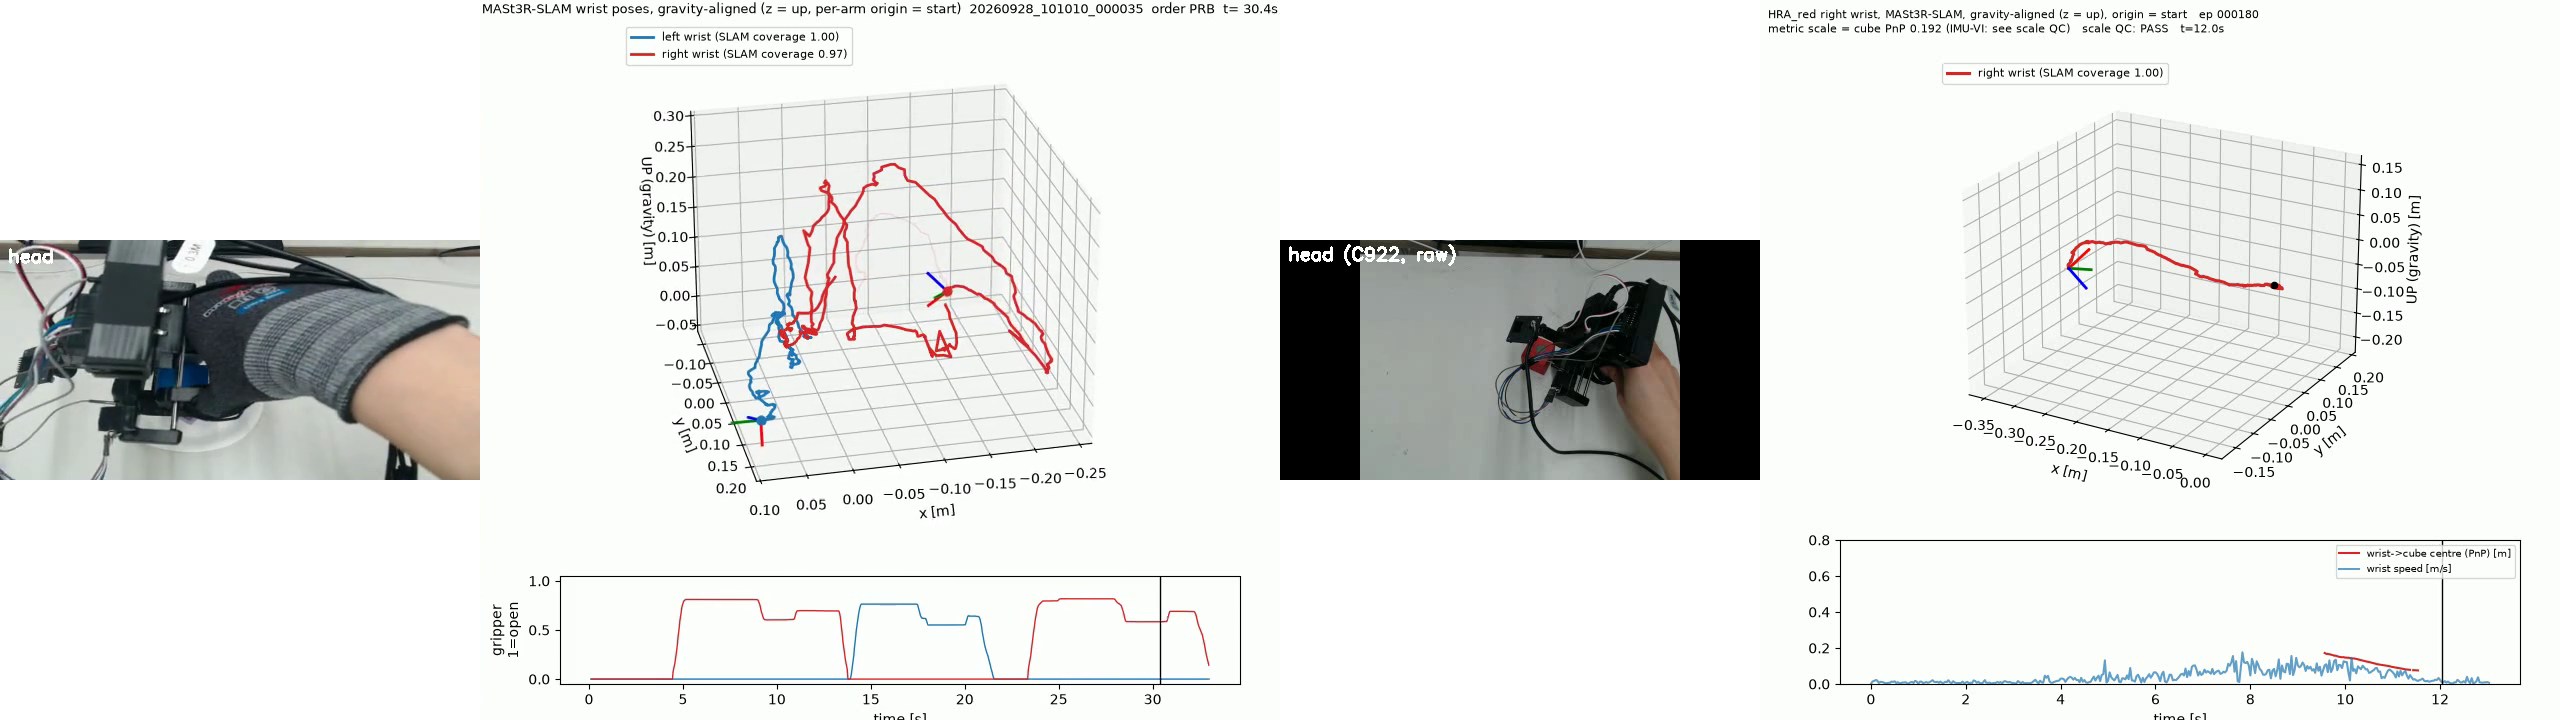
\includegraphics[width=0.8\textwidth]{../figures/fig7_mast3r_trajectories.png}
\caption{HRL80 쌓기 테이크(순서 PRB)의 MASt3R-SLAM 손목 궤적. 왼쪽: 헤드 카메라와 두 손목 어안 카메라. 오른쪽: 중력 정렬(z 위쪽)된
궤적으로, 각 팔의 원점은 시작 자세이고 현재 공구 축을 표시(x 빨강, y 초록, z 파랑)하며 메트릭 스케일은 IMU에서 얻었다. 아래: 두
그리퍼(1 = 열림). 세 테이크(PRB, RBP, PBR)의 영상은 저장소의
\texttt{docs/media/mast3r\_trajectories/hrl80\_0000\{35,55,60\}\_wrist.mp4}에 있다.}
\label{fig:traj}
\end{figure*}

\textbf{데이터.} 원천은 손별 IMU 스케일이 유효한 원래 에피소드 273개와 HRL80 에피소드 60개이다. HRL80 에피소드 3개는 한 손의 IMU
스케일이 유효하지 않아 제외되어 330개가 남는다. 로봇 작업공간이나 IK 실현 가능성으로는 아무것도 필터링하지 않는다. 15\,Hz 행
111{,}533개 중 57{,}283개(51.4\%)가 학습에 사용 가능하며, 나머지는 추적 손실, 동기화 공백, 또는 에피소드의 마지막 0.8\,s에 걸린다.
분할은 이전 릴리스에서 고정한 것을 쓴다(검증 = \ref{sec:proc}절의 held-out 에피소드 26개와 HRL80 에피소드 49--54). 학습 에피소드 298개에
행 51{,}612개, 검증 에피소드 32개에 행 5{,}671개이다.

\textbf{드러나지 않는 자세 점프.} 에고와 로봇의 상태 통계를 비교한 결과, 로봇 데이터에는 없는 행당 100\mm 초과의 상태 점프가 에고
데이터에 있었다. 두 원인이 섞여 있었다. 첫째, 내보낸 데이터셋에는 학습 행만 있으므로 ``인접'' 프레임이 수 초 떨어져 있을 수 있다.
30\mm{}를 넘는 겉보기 점프 2{,}598개 중 1{,}482개(57\%)가 이런 시간 공백이며, 인접 여부는 행 타임스탬프로 판단해야 한다. 둘째, 나머지
점프는 실제이다. MASt3R-SLAM은 추적 손실을 표시하지 않은 채 30\,Hz 한 프레임 안에서 카메라를 10\,cm 이상 옮기는 경우가 가끔 있다(학습
에피소드 24개에서 3\,m/s보다 빠른 원시 스텝 55개, 그 어느 것도 앞서 손실 플래그가 없었다). 상태는 과제 시작에 앵커링되어 있으므로 한
방향 점프는 그 에피소드의 이후 모든 상태를 손상시키는 반면, 현재 시점에 앵커링된 액션은 0.8\,s 동안만 영향을 받는다. v2b 필터는 한 방향
점프(행당 100\mm 또는 45\textdegree{} 초과, 또는 느린 두 스텝 사이의 고립된 50\mm 초과 스텝) 이후 에피소드의 나머지를 버리고, 고립된
스파이크는 그 스파이크만 버린다. 이 필터는 학습 에피소드 42개의 이벤트 44건에 작용하며 에피소드 하나를 통째로 제거한다. 학습은 에피소드
297개, 행 48{,}411개($-6.20$\%)로 줄고 검증은 변하지 않는다. 시간상 인접한 행 사이의 최대 스텝은 422.5에서 90.5\mm{}로, 100\mm 초과
스텝은 18개에서 0개로 줄며, 3\,m/s보다 빠른 원시 스텝 7개는 유효 행 안에 남는다.

\textbf{에고 데이터와 로봇 데이터의 차이.} 에고 에피소드 60개와 로봇 에피소드 60개에서, 에고 자세를 로봇 시작 자세에 붙였을 때 로봇
IK는 에고 위치의 99.7\%(왼쪽)와 99.5\%(오른쪽), 에고 전체 자세의 72.3\%/74.6\%에 도달한다. 로봇에서 쓰는 IK 구성은 손목 관절 하나를
잠그므로 로봇 \emph{자신의} 기록 자세도 45.2\%/52.2\%만 재현하는데, 이는 인간 데이터와 무관하게 존재하는 배포상의 한계이다. 에고 손은
더 작은 작업공간을 쓰고(상태 p95 0.221/0.214\,m 대 0.395/0.369\,m), 0.4\,s 이동량은 비슷하며(p95 93/99 대 91/100\mm), 에고는 두 손이
동시에 정지해 있는 경우가 훨씬 잦다(0.4\,s 기준 샘플의 19.5\% 대 2.4\%). 가장 큰 차이는 시각적이다. 선명도 척도인 이미지 Laplacian의
분산 중앙값이 에고 손목 어안 시점에서는 1{,}854/1{,}487, 로봇 손목 카메라에서는 59/64이다.

\section{전이 실험}\label{sec:transfer}
이 절의 모든 실행은 하나의 레시피를 공유한다. 32-D 액션 헤드를 쓰는 X-VLA로, 손실은 액션 차원 0--19에만 걸고 차원 20--31은 입력과
출력에서 0으로 두며, 배치 8, 8-bit AdamW(정책 학습률 $10^{-4}$, warm-up 1k, 마지막 스텝에서 끝나는 cosine decay), bf16 혼합 정밀도,
seed 1000이다. 로봇 데이터는 같은 여섯 순서 쌓기 과제의 원격조작 에피소드 312개(프레임 174{,}012개)인 R312c이다. 파인튜닝은 새
옵티마이저로 시작하며 로봇 정규화 통계를 쓴다.

\textbf{어떤 soft prompt인가?} X-VLA는 soft prompt 집합을 선택하는 데이터셋/embodiment id를 조건으로 받는다. 이전 실행은 id~0을
썼다. 공개 base 가중치를 읽어 보면 슬롯 10--17만 학습되었다. 나머지 22개 슬롯에서는 인코더와 디코더 bias가 정확히 0이고 프롬프트
가중치가 초기값 근처에 머문다. 따라서 본 연구에서 쓴 id 0과 6은 모두 학습되지 않은 슬롯이었다. 학습된 슬롯이 더 나은 출발점인 것도
아니다. R312c에서의 초기 손실은 슬롯 0이 1.11, 6이 1.12, 15가 1.61, 10이 2.35, 16이 2.65, 17이 4.07, 11이 22.80이다. 아래의 모든 실행은
사용되지 않은 슬롯 20을 본 embodiment 전용 슬롯으로 쓴다.

\textbf{로봇 프레임에서의 에고 전용 모델.} 에고 데이터만으로 40k 스텝 학습한 뒤, 모델을 teacher forcing 방식으로 로봇 프레임 120개에
질의하고, 로봇 데이터로 40k 스텝 학습한 모델과 비교하였다(이 프레임들은 후자 모델의 학습 세트에 포함되므로 그 값은 상한 기준이다).
0.4\,s에서 예측 이동과 기록 이동 사이 코사인 중앙값은 로봇 모델이 $+0.81$/$+0.77$(왼쪽/오른쪽), 에고 모델이 $-0.05$/$-0.03$이다.
좌우 교환과 축 부호 반전의 어떤 조합도 에고 모델을 $+0.16$ 위로 올리지 못하며, 손목 카메라 광류(optical flow)는 두 도메인에서 TCP
동작과 같은 부호 관계를 가지므로, 이는 규약 오류가 아니다.

\begin{table}[t]
\centering\footnotesize\setlength{\tabcolsep}{3.2pt}
\caption{에고 전용 체크포인트(40k)에서 이미지와 상태가 서로 다른 도메인에서 올 때의 $k{=}4/8/16$ 방향 코사인 중앙값(왼쪽 $|$ 오른쪽).
에고 검증 프레임 100개와 로봇 프레임 100개, 셀당 동작 프레임 21--55개.}
\label{tab:ablation}
\begin{tabular}{@{}lcc@{}}
\toprule
이미지 + 상태 & 왼쪽 $k$=4/8/16 & 오른쪽 $k$=4/8/16 \\
\midrule
에고 + 에고 & 0.87 / 0.91 / 0.92 & 0.89 / 0.94 / 0.84 \\
에고 + 0 & 0.77 / 0.80 / 0.89 & 0.85 / 0.80 / 0.66 \\
에고 + 로봇 & 0.76 / 0.81 / 0.90 & 0.72 / 0.69 / 0.72 \\
로봇 + 로봇 & 0.36 / 0.30 / $-$0.01 & 0.19 / 0.02 / $-$0.15 \\
로봇 + 0 & 0.17 / 0.25 / $-$0.25 & 0.24 / 0.06 / $-$0.02 \\
로봇 + 에고 & 0.16 / 0.24 / $-$0.16 & 0.49 / 0.33 / $-$0.03 \\
\bottomrule
\end{tabular}
\end{table}

\textbf{격차는 이미지에 있다.} 표~\ref{tab:ablation}는 두 입력을 맞바꾼다. 에고 이미지를 주면 모델은 로봇 상태를 포함해 어떤 상태가
주어지든 0.69--0.90의 코사인을 유지하고, 로봇 이미지를 주면 상태와 관계없이 $-0.25$에서 $+0.49$ 사이로 떨어진다. 실패는 시각적이며,
이는 손목 시점의 30배 선명도 차이와 부합한다.

\textbf{초기값으로서의 에고 사전학습.} R312c에서 base 모델(A)과 50k 스텝 에고 모델(B)로부터 동일한 데이터, 스케줄(150k 스텝 cosine),
시드, 레시피로 파인튜닝하였다. 두 실행 모두 60k 근처에서 직접 중단하였다. 스텝 200에서 학습 손실은 A가 0.945, B가 0.244이다. 비율 B/A는
처음 5k 스텝에서 0.49, 5k--20k에서 0.875, 20k--40k에서 0.95이며, 55k--60k에서는 두 값이 동률이다(0.0733 대 0.0745, 기록된 24개 지점
중 13개에서 B가 낮음)(그림~\ref{fig:egoinit}). 따라서 에고 사전학습은 로봇 데이터의 초기 피팅을 빠르게 하지만, 60k까지 학습 손실에서
측정 가능한 이점을 주지 않는다. 이는 조건당 시드 하나의 학습 손실이며, A와 B의 held-out 또는 폐루프 비교는 없다. 이후 300k 실행 두 개가
끝났으나 서로 다른 로봇 데이터셋(에고 초기화 실행은 R312c, scratch 실행은 에피소드 384개)을 썼으므로 전이 비교가 아니며, 전이 비교로
보고하지 않는다.

\begin{figure*}[t]
\centering
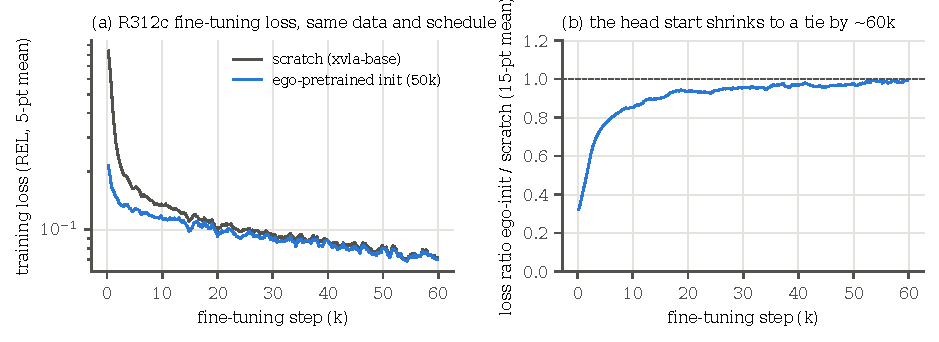
\includegraphics[width=\textwidth]{../figures/fig5_ego_init_loss.pdf}
\caption{같은 데이터·스케줄·시드에서 base 모델과 50k 에고 체크포인트로부터의 R312c 파인튜닝 비교. (a) 학습 손실. (b) 둘의 비율.
1 미만이면 에고 초기화에 유리하다. 학습 손실만 해당.}
\label{fig:egoinit}
\end{figure*}

\textbf{시각적 격차를 줄이려는 시도.} 에고 손목 시점을 로봇처럼 보이게 하기 위해, 각 어안 프레임을 가상 핀홀 카메라(수평 화각
62--70\textdegree{}, 로봇처럼 조가 이미지 아래쪽에 오도록 주점을 이동)로 다시 렌더링한 뒤 다운샘플링, 블러, JPEG 압축을 적용한다.
레이블, 상태, 헤드 이미지는 바꾸지 않는다. 모든 프레임에 적용하면(ROBOT100) 손목 선명도 중앙값은 1{,}854/1{,}487에서 181/132로
떨어지지만, 여전히 로봇의 59/64보다 2--3배 높다. 프레임의 70\%를 다시 렌더링한 실행은 5k 스텝에서 중단하였고, 배치마다 정확히 에고
(ROBOT100) 샘플 4개와 로봇 샘플 4개를 쓰는 공동 학습 실행은 평가 없이 88.6k 스텝에서 중단하였다. 300k ROBOT100 사전학습 실행(에피소드
297개, 행 48{,}411개, 49.6 epoch)은 10월 5일 학습 손실 0.007로 끝났으며, 그 체크포인트들이 \ref{sec:r30}절의 에고 초기값이다. 다시
렌더링한 모델에 대해서는 오프라인 전이 지표를 계산하지 않았다.

\textbf{로봇에서.} 위 모든 실행의 체크포인트를 배포 인터페이스를 통해 reBot에서 실행하였다. 10월 2일에서 4일 사이에 체크포인트 71개,
제어 사이클 49{,}431회, 실행 시작 1{,}681회이다. 사이클 로그는 과제 결과가 아니라 모델 자신의 웨이포인트에 대한 IK 추적을 기록하며,
에피소드나 지시문 필드가 없어 성공률을 산출할 수 없다. 조작자의 관찰 두 가지는 로그로 남지 않았다. 첫째, 파인튜닝 10k 스텝의 에고 초기화
모델은 큐브를 잡았으나 틀린 색을 집었다. 둘째, R312c로 300k 파인튜닝한 에고 초기화 모델(B300, 75k에서 205k 사이의 체크포인트)이
로봇에서 폐루프로 큐브 세 개를 끝까지 쌓았다. 시도 횟수는 기록되지 않았고 영상도 찍지 않았으므로, 폐루프 큐브 삼단 쌓기가 시연되었다는
사실만 말할 수 있으며 성공률은 없다. 이는 에고 사전학습의 가치에 대해서도 아무것도 말해 주지 않는다. 같은 R312c 데이터로 학습한
scratch 모델은 같은 프로토콜로 평가되지 않았다(완료된 scratch 300k 실행은 R384를 사용). 10월 5일에서 7일 사이 양팔 로봇 사용은 R384
scratch 모델(200k, 제어 사이클 4회)의 짧은 실행 한 번뿐이었다. \ref{sec:lim}절에 나열한 필드를 갖춘 시도 로거가 10월 4일 배포
인터페이스에 추가되었으나 사용되지 않았으므로, 기록된 시도 결과는 여전히 없다. 10월 4일 저장소 정리에서 50k의 배수인 체크포인트만
남겼다. 큐브를 쌓은 B300 체크포인트 중 150k와 200k는 남아 있고 나머지(155k--205k)는 사라졌으므로, 시연은 150k 또는 200k에서만 재현할
수 있다.

\section{저데이터 Ablation: 로봇 에피소드 30개}\label{sec:r30}
\ref{sec:transfer}절의 312 에피소드 비교는 로봇 데이터가 초기값의 영향을 씻어 낼 여지를 충분히 준다. 인간 데이터 활용에 중요한 질문은
로봇 데이터가 부족할 때 도움이 되는지이다. 따라서 R312c의 에피소드 150--179인 R30(에피소드 30개, 프레임 17{,}600개, 쌓기 순서당 5개)으로,
\ref{sec:transfer}절의 레시피, R312c 정규화 통계, seed 1000, 600k 스텝 cosine 스케줄을 써서 세 초기값에서 파인튜닝하였다. base 모델
(scratch)과, \ref{sec:transfer}절의 ROBOT100 에고 사전학습 실행의 100k 및 300k 스텝이다. 100k 체크포인트는 같은 300k 스텝 스케줄의 중간에서
가져온 것이므로 학습률이 감쇠하지 않은 상태이며, 별도의 100k 스텝 실행이 아니다. 또한 두 에고 조건은 서로 다른 기계에서 실행되었으므로
(scratch와 100k-init은 RTX~4090, PyTorch~2.6; 300k-init은 RTX~5090, PyTorch~2.7.1) 비트 단위로 동일한 쌍둥이 실행이 아니다.

\begin{table}[t]
\centering\footnotesize\setlength{\tabcolsep}{4pt}
\caption{R30 파인튜닝, 맞춘 스텝에서의 학습 손실(200스텝 이동 평균)과 scratch 대비 윈도 평균의 비율(1 미만이면 에고 초기화에 유리).
조건당 시드 하나, held-out 또는 로봇 평가 없음.}
\label{tab:r30}
\begin{tabular}{@{}lccc@{}}
\toprule
스텝 & Scratch & Ego-PT 100k 초기화 & Ego-PT 300k 초기화 \\
\midrule
200 & 0.801 & 0.239 & 0.446 \\
1k & 0.312 & 0.103 & 0.117 \\
10k & 0.065 & 0.056 & 0.040 \\
50k & 0.019 & 0.017 & 0.014 \\
100k & 0.009 & 0.009 & 0.007 \\
\midrule
윈도 & & 비율 & 비율 \\
\midrule
1k--5k & & 0.544 & 0.493 \\
10k--20k & & 0.823 & 0.697 \\
50k--100k & & 0.970 & 0.856 \\
100k--150k & & 1.021 & 0.914 \\
\bottomrule
\end{tabular}
\end{table}

\textbf{결과.} 표~\ref{tab:r30}와 그림~\ref{fig:r30}은 312 에피소드 비교와 같은 양상을 더 길게 늘여 보여 준다. 두 에고 초기화 모두 scratch
손실의 절반 미만에서 출발한다(1k--5k 윈도 비율 0.54와 0.49). 100k 스텝 초기화는 약 100k 스텝까지 이점을 잃고(50k--100k 비율 0.97,
100k--150k 비율 1.02), 300k 스텝 초기화는 더 작은 이점을 더 오래 유지하며(0.86과 0.91) 약 200k에서 동등해진다. 약 150k 이후로는 모든
손실이 출력 정밀도에서 0.001--0.004이므로 비율은 의미가 없다. 100k 스텝 초기화는 사전학습을 덜 했음에도 300k 스텝 초기화보다 낮게
출발하는데(스텝 200에서 0.239 대 0.446), 그 이유는 아직 설명하지 못했다. 세 실행 모두 GPU를 비우기 위해 471k(scratch), 305k(100k-init),
310k(300k-init)에서, 즉 214, 139, 141 epoch 후에 직접 중단하였다. 에피소드가 30개뿐이어서 모든 조건이 스케줄이 끝나기 훨씬 전에 학습
데이터에 거의 정확히 맞는다.

\textbf{이 결과가 보여 주는 것과 보여 주지 않는 것.} 30개 에피소드에서의 학습 손실은 각 초기값이 로봇 데이터를 얼마나 빨리 암기하는지를
측정할 뿐, 얼마나 잘 행동하는지를 측정하지 않는다. 모든 조건이 심하게 과적합하므로, 의미 있는 비교는 초기값 간 차이가 아직 남아 있는
초·중반 체크포인트(대략 10k--150k)에서의 폐루프 비교이다. 그러나 R30 체크포인트는 아직 로봇에서 실행되지 않았고 held-out 로봇 평가도
없다. 이 실험이 검증할 수 있는 예측은 에고 초기화 모델의 빠른 피팅이 더 적은 파인튜닝 스텝에서의 쌓기 성공으로 이어지는지이며, 이 실험은
아직 수행되지 않았다.

\begin{figure*}[t]
\centering
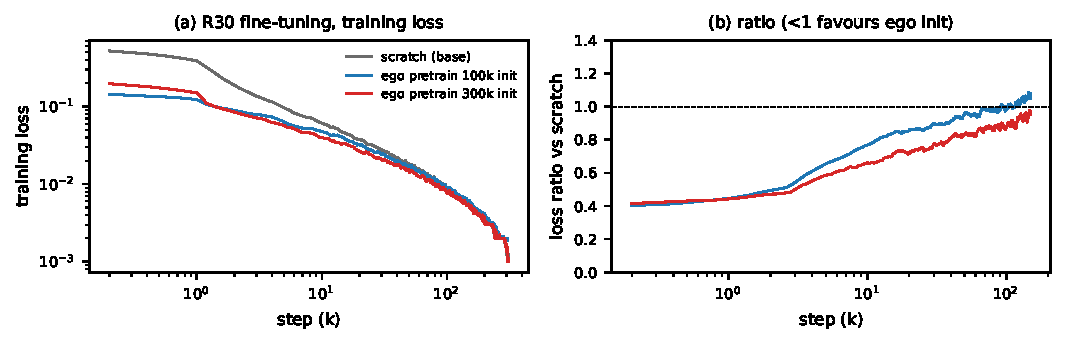
\includegraphics[width=0.8\textwidth]{../figures/fig8_r30_ablation.pdf}
\caption{base 모델과 100k·300k 스텝 에고 사전학습으로부터의 R30 파인튜닝(로봇 에피소드 30개). (a) 학습 손실(log--log, 평활화).
(b) scratch 대비 비율, 150k까지 표시. 그 이후는 소수점 셋째 자리 손실 때문에 비율이 노이즈가 된다. 학습 손실만 해당, 조건당 시드 하나.}
\label{fig:r30}
\end{figure*}

\section{교훈}\label{sec:lessons}
네 가지 발견이 작업 방식을 바꾸었으며, 각각은 손실 곡선이 아니라 명시적인 검사로 발견되었다. (i) 사전학습 모델의 조건화 인터페이스는
가정하지 말고 점검해야 한다. 본 연구의 embodiment id 두 개는 한 번도 학습된 적 없는 soft prompt를 가리키고 있었다. (ii) 인간 데이터와
로봇 데이터가 텐서 계약을 공유하면, 도메인 간 입력을 맞바꾸어 남은 격차의 위치를 찾을 수 있다. 여기서는 기구학이나 정규화가 아니라 손목
이미지였다. (iii) 모든 스케일 또는 자세 원천에는 드러나지 않게 실패하는 영역이 있다. 여기서는 드문 한 프레임 점프에서의 MASt3R-SLAM,
제2부에서는 느린 동작에서의 IMU 스케일이다. 두 경우 모두 독립적인 기준(로봇 통계, 알려진 물체)과 비교해서만 잡혔으며, 이제 이를 모든
새 수집에 포함한다. (iv) 초기값 간 학습 손실 비교는 로봇 데이터가 거의 0까지 피팅될 때마다 동률로 끝난다. 312개와 30개 에피소드 모두
그랬다. 이점은 초기 체크포인트에서의 held-out 또는 폐루프 평가로만 보일 수 있으며, 이를 위한 로깅은 로봇 실행 후가 아니라 그 전에
갖춰져 있어야 한다.

\section{한계 및 향후 연구}\label{sec:lim}
\textbf{완료:} 데이터셋 수집과 캘리브레이션, 자세·리타게팅·QA 파이프라인, 300k 스텝 에고 파인튜닝과 held-out 에피소드 오프라인 평가,
리타게팅 v2, 로봇 유사 재수집, 150 에피소드 로봇 파인튜닝 맞춤 비교, 최종 996 세그먼트 데이터셋 사전학습(211.7k 스텝에서 중단,
체크포인트 100k와 200k). 버전 3에서 데카르트 에고 데이터셋과 필터, soft prompt 점검, 도메인 교환 진단, 60k 스텝까지의 초기값 맞춤 비교,
로봇 유사 손목 재렌더링을 추가하였다. 버전 4에서 완료된 ROBOT100 사전학습과 세 조건 R30 ablation(학습 손실, 305k--471k에서 중단)을
추가하였다. \textbf{조기 중단, 결론 없음:} 버전 2의 90, 60, 30 에피소드 로봇 파인튜닝 비교(맞춘 스텝 최대 두 개, 또는 한 조건만 실행),
70\% 재렌더링 사전학습(5k 스텝), 에고/로봇 공동 학습 실행(88.6k 스텝, 평가하지 않음).
\textbf{미수행:} 996 세그먼트 체크포인트로부터의 로봇 파인튜닝, R30 조건들의 로봇 또는 held-out 평가, 에고 초기화 모델과 scratch 모델의
held-out 또는 폐루프 비교, 로봇에서의 결과 로깅(로거는 있으나 기록된 시도가 없음). 버전 2의 로봇 평가 에피소드는 파인튜닝 데이터와
겹치므로, 겹치지 않는 로봇 데이터에서의 이점은 아직 보여야 한다.

\textbf{본 연구가 뒷받침하지 않는 것:} (i) 폐루프 성공률(로봇 에피소드 312개로 파인튜닝한 모델로 큐브 삼단 쌓기가 시연되었으나 시도
횟수를 세지 않음), 또는 에고 초기화 모델과 scratch 모델 간의 폐루프 차이, (ii) 새 큐브 배치로의 일반화(배치를 기록하지 않았고 설계상
절대 기하를 버림), (iii) 보지 못한 쌓기 순서로의 일반화(여섯 순서 모두 학습에 등장), (iv) 조작자 한 명, 장면 하나, 사흘을 넘어서는 전이,
(v) 로봇 학습 분포를 더 빨리 피팅하는 것 이상의 인간 데이터 이점, (vi) 에고 전용 정책 또는 재렌더링한 손목 이미지가 로봇 카메라로 전이된다는
것. \textbf{계획된 실험:} 모든 로봇 시도를 기록하고(모델, 체크포인트, 로봇 데이터 크기, 배치, 지시문, 쌓기 단계 0--3, 틀린 색, 실패 원인)
모델당 20--30회 시도한다. scratch 모델과 에고 초기화 모델을 맞춘 파인튜닝 스텝과 축소된 로봇 데이터(에피소드 30개)에서 비교하여 쌓기가
처음 성공하는 스텝 및 데이터 예산을 찾는다. 헤드 카메라로 배치를 기록하고 배치 영역을 held-out으로 둔다. 두 순서를 완전히 held-out으로
두고 지시문 추종을 검증한다. 정지 구간을 고려한 손실이나 가중치로 학습한다. 순서 지시문을 통제 변수로 하여 로봇에서 폐루프로 평가한다.

더 넓게 보면, 본 연구는 에고센트릭 인간 시연이 로봇 정책에 확장 가능한 지도 신호를 제공하는 연구 의제를 향한 첫걸음이다. 즉 embodiment
세부는 버리고 과제 기하와 의도는 유지하는 인간--로봇 표현을 학습하고, 실행 전에 예측 world model로 이를 평가하는 것이다. 현재 결과는
병목이 정책 못지않게 자세 복원, 필터링, 평가 설계에 있음을 보여 준다.

\section{결론}
큐브 삼단 쌓기의 양팔 에고센트릭 시연 349개를 수집하고, 게이트 기반 파이프라인으로 로봇 관절 공간 세그먼트 561개로 처리한 뒤, 그 결과로
0.9B VLA를 파인튜닝하였다. 오프라인에서 모델은 동작 샘플에 대해 held-out 인간 동작의 방향을 안정적으로 예측하고($k{=}30$에서 코사인
0.90) 무동작 기준선 대비 관절 공간 오차를 줄인다(구간에 따라 13--32\%). 정지 샘플에서는 허위 동작을 예측하며, 집계 지표는 이를 가리고,
순서 지시문을 바꾸어도 예측이 더 정확해지지 않는다. 다중 시드 궤적 검색은 리타게팅 손실의 상당 부분을 없애며, 에고 사전학습은 로봇
데이터로 파인튜닝할 때 작지만 일관된 이득을 주는데, 이는 로봇 학습 에피소드에서 측정한 것이다. 에피소드 전체를 로봇의 데카르트 액션 계약으로
변환하면, 드러나지 않는 SLAM 점프에 대한 필터를 거친 뒤 실현 가능성 필터 없이 에피소드 330개가 남는다. 이 계약 아래에서 남은 인간--로봇
격차는 시각적이다. 에고 전용 모델은 로봇 카메라 프레임에서 유용한 액션 방향을 주지 못하며, 격차는 상태가 아니라 손목 이미지를 따른다.
초기값으로서 에고 사전학습은 초기 로봇 파인튜닝을 빠르게 하고, 학습 손실상의 이점은 60k 스텝에서 사라진다. 로봇 에피소드 312개로
파인튜닝한 에고 초기화 모델이 로봇에서 큐브 세 개를 끝까지 쌓았으므로 과제 자체는 폐루프로 해결되었다. 에고 사전학습이 더 적은 로봇
에피소드나 더 적은 파인튜닝 스텝으로 그 지점에 도달하는지는 열린 질문이다. 느린 단일 팔 동작에서는 알려진 물체가 IMU 스케일을 대신한다.
공간 및 과제 순서 일반화, 겹치지 않는 로봇 데이터에서의 이점, 측정된 성공률에는 위에 나열한 통제 실험이 필요하다. 로봇 에피소드 30개에서도
에고 사전학습은 초기 피팅을 빠르게 하고, 사전학습이 길수록 더 오래 그러하며, 역시 학습 손실상의 이점은 사라진다. 그것이 초기
체크포인트에서 폐루프 이점이 되는지가 다음 실험이다.

\begin{thebibliography}{99}\footnotesize
\bibitem{chi2024umi} C.~Chi, Z.~Xu, C.~Pan, E.~Cousineau, B.~Burchfiel, S.~Feng, R.~Tedrake, and S.~Song, ``Universal manipulation interface: In-the-wild robot teaching without in-the-wild robots,'' in \emph{RSS}, 2024.
\bibitem{wang2024dexcap} C.~Wang, H.~Shi, W.~Wang, R.~Zhang, L.~Fei-Fei, and C.~K. Liu, ``DexCap: Scalable and portable mocap data collection system for dexterous manipulation,'' in \emph{RSS}, 2024.
\bibitem{kareer2024egomimic} S.~Kareer \emph{et al.}, ``EgoMimic: Scaling imitation learning via egocentric video,'' \emph{arXiv:2410.24221}, 2024.
\bibitem{wang2023mimicplay} C.~Wang \emph{et al.}, ``MimicPlay: Long-horizon imitation learning by watching human play,'' in \emph{CoRL}, 2023.
\bibitem{grauman2022ego4d} K.~Grauman \emph{et al.}, ``Ego4D: Around the world in 3,000 hours of egocentric video,'' in \emph{CVPR}, 2022.
\bibitem{zhao2023act} T.~Z. Zhao, V.~Kumar, S.~Levine, and C.~Finn, ``Learning fine-grained bimanual manipulation with low-cost hardware,'' in \emph{RSS}, 2023.
\bibitem{chi2023diffusion} C.~Chi, S.~Feng, Y.~Du, Z.~Xu, E.~Cousineau, B.~Burchfiel, and S.~Song, ``Diffusion policy: Visuomotor policy learning via action diffusion,'' in \emph{RSS}, 2023.
\bibitem{kim2024openvla} M.~J. Kim \emph{et al.}, ``OpenVLA: An open-source vision-language-action model,'' in \emph{CoRL}, 2024.
\bibitem{black2024pi0} K.~Black \emph{et al.}, ``$\pi_0$: A vision-language-action flow model for general robot control,'' \emph{arXiv:2410.24164}, 2024.
\bibitem{zheng2025xvla} J.~Zheng \emph{et al.}, ``X-VLA: Soft-prompted transformer as scalable cross-embodiment vision-language-action model,'' in \emph{ICLR}, 2026 (arXiv:2510.10274).
\bibitem{cadene2024lerobot} R.~Cadene \emph{et al.}, ``LeRobot: State-of-the-art machine learning for real-world robotics in PyTorch,'' \url{https://github.com/huggingface/lerobot}, 2024.
\bibitem{lipman2023flow} Y.~Lipman, R.~T.~Q. Chen, H.~Ben-Hamu, M.~Nickel, and M.~Le, ``Flow matching for generative modeling,'' in \emph{ICLR}, 2023.
\bibitem{murai2025mast3rslam} R.~Murai, E.~Dexheimer, and A.~J. Davison, ``MASt3R-SLAM: Real-time dense SLAM with 3D reconstruction priors,'' in \emph{CVPR}, 2025.
\bibitem{furgale2013kalibr} P.~Furgale, J.~Rehder, and R.~Siegwart, ``Unified temporal and spatial calibration for multi-sensor systems,'' in \emph{IROS}, 2013.
\bibitem{xiao2024florence2} B.~Xiao \emph{et al.}, ``Florence-2: Advancing a unified representation for a variety of vision tasks,'' in \emph{CVPR}, 2024.
\end{thebibliography}
\end{document}
